% SIAM Article Template
\documentclass[review,hidelinks,onefignum,onetabnum]{siamart220329}

% Information that is shared between the article and the supplement
% (title and author information, macros, packages, etc.) goes into
% ex_shared.tex. If there is no supplement, this file can be included
% directly.

% SIAM Shared Information Template
% This is information that is shared between the main document and any
% supplement. If no supplement is required, then this information can
% be included directly in the main document.


% Packages and macros go here
\usepackage{lipsum}
\usepackage{amsfonts}
\usepackage{graphicx}
\usepackage{epstopdf}
\usepackage{algorithmic}
\usepackage{amsmath}
%\usepackage{natbib}
\ifpdf
  \DeclareGraphicsExtensions{.eps,.pdf,.png,.jpg}
\else
  \DeclareGraphicsExtensions{.eps}
\fi

% Add a serial/Oxford comma by default.
\newcommand{\creflastconjunction}{, and~}

% Used for creating new theorem and remark environments
\newsiamremark{remark}{Remark}
\newsiamremark{hypothesis}{Hypothesis}
\crefname{hypothesis}{Hypothesis}{Hypotheses}
\newsiamthm{claim}{Claim}

% Sets running headers as well as PDF title and authors
\headers{An Example Article}{D. Doe, P. T. Frank, and J. E. Smith}

% Title. If the supplement option is on, then "Supplementary Material"
% is automatically inserted before the title.
\title{Restarting the non-symmetric Lanczos algorithm via the implicitly shifted LR algorithm\thanks{Submitted to the editors DATE.
\funding{This work was funded by the Fog Research Institute under contract no.~FRI-454.}}}

% Authors: full names plus addresses.
\author{P. S. Negi\thanks{Imagination Corp., Chicago, IL 
  (\email{prabal.negi@su.se}, \url{http://www.imag.com/\string~ddoe/}).}
\and C. Arratia\thanks{Department of Applied Mathematics, Fictional University, Boise, ID 
  (\email{cristobal.arratia@su.se}).}
}

\usepackage{amsopn}
\DeclareMathOperator{\diag}{diag}


%%% Local Variables: 
%%% mode:latex
%%% TeX-master: "ex_article"
%%% End: 


% Optional PDF information
\ifpdf
\hypersetup{
  pdftitle={An Example Article},
  pdfauthor={D. Doe, P. T. Frank, and J. E. Smith}
}
\fi

\newcommand{\Citation}{(\textbf{Citation}) }

\newcommand{\refeqn}[1]{equation~(\ref{#1})}

\newcommand{\bracketref}[1]{~(\ref{#1})}

%\floatname{algorithm}{Procedure}
%\renewcommand{\algorithmicrequire}{\textbf{Input:}}
%\renewcommand{\algorithmicensure}{\textbf{Output:}}


% The next statement enables references to information in the
% supplement. See the xr-hyperref package for details.

\externaldocument[][nocite]{ex_supplement}

% FundRef data to be entered by SIAM
%<funding-group specific-use="FundRef">
%<award-group>
%<funding-source>
%<named-content content-type="funder-name"> 
%</named-content> 
%<named-content content-type="funder-identifier"> 
%</named-content>
%</funding-source>
%<award-id> </award-id>
%</award-group>
%</funding-group>

\begin{document}

\maketitle

% REQUIRED
\begin{abstract}
The shifted QR iteration is used as a restart procedure for the Arnoldi method for the calculation of a few dominant eigenvalues of a large matrix. We show that the underlying idea can be utilized in much the same manner via the shifted LR iteration to create a restart procedure for the non-symmetric Lanczos algorithm for eigenvalue calcuations. Additionally, we show that the (shifted) LR iteration can be performed implicitly in a manner similar to the Francis' algorithm, resulting in a bulge-chase type procedure which does not require the explicit construction of the full lower and upper triangular matrices. 
\end{abstract}

% REQUIRED
\begin{keywords}
LR algorithm, unsymmetric Lanczos, implicit restart
\end{keywords}

% REQUIRED
\begin{MSCcodes}
68Q25, 68R10, 68U05
\end{MSCcodes}

\section{Introduction}
The Arnoldi iteration \cite{arnoldi51} is a popular Krylov space method for calculating a few eigenvalues of a large matrix. The method relies on the generation of a sequence of Krylov vectors which determine the subspace within which approximations of the eigenvalue-eigenvector pairs are obtained. Depending on the accuracy and number of eigenpair approximations needed, the Krylov space size can become exceedingly large so that  the quality of the results may be limited by the available memory. Sorensen \cite{sorensen92} introduced an elegant procedure for restarting the Arnoldi factorization based on polynomial filters, which are applied through the implicitly shifted QR iterations on the reduced Hessenberg matrix obtained through the Arnoldi method. In particular, the use of exact shifts was shown to be successful in the convergence process of the eigenspace\cite{sorensen92} of the specified eigenvalues. The method has subsequently found widespread application through the ARPACK library \cite{arpack98}. The use of QR iterations ensures that the reduced matrix preserves its Hessenberg structure through the transforms that make up the restart process. If the underlying matrix is symmetric, the Arnoldi iteration reduces to the Lanczos algorithm and, the Hessenberg matrix reduces to a symmetric tridiagonal matrix. The QR iteration preserves the symmetric tridiagonal structure as well and, as pointed out by Sorensen \cite{sorensen92}, the implicit restart process applies equally well for the Lanczos method for symmetric matrices. 

One would like to extend this procedure to the case of the non-symmetric Lanczos method. However, the reduced matrix that one obtains is a non-symmetric tridiagonal matrix, with the tridiagonal structure being the result of the recurrence relations of the Lanczos algorithm \cite{saad82}. Since the QR iterations do not preserve the banded structure of non-symmetric matrices, a straightforward application of the restart procedure propounded by Sorensen will lead to a loss of this tridiagonal structure of the reduced matrix (the Hessenberg structure will still be preserved).  This loss of structure can be circumvented if one looks to the predecessor of the QR algorithm namely, the LR algorithm proposed by Rutihauser \cite{rutishauser58,rutishauser63,rutihauser91}, which has the attractive property of preserving the band structure of a matrix. This property was already pointed out by Rutihauser in \cite{rutishauser58} where the banded matrices were referred to as striped matrices. As we will show in the next section, the shifted LR transform is the appropriate generalization of the restart procedure to the case of non-symmetric Lanczos iteration. The process would necessarily require refining both the right as well as the left Krylov spaces simultaneously.

The rest of the paper is organized as follows. In the next section we start with the introduction of the non-symmetric Lanczos iteration and then develop the restart procedure. We also show that the LR algorithm can be implemented as a bulge-chase method, similar to the Francis' algorithm. In section 3 we apply the restart process to the Grcar matrix, and make some concluding remarks in section 4.

\section{Non-symmetric Lanczos}
Lanczos first introduced his algorithm in \cite{lanczos50} as a method for tridiagonalizing a matrix, but also realized that the method could be used iteratively to find eigenvalues. For an arbitry matrix $A$, the method generates a pair of Krylov subspaces $\{v_{1},\ldots,v_{j}\}$ and $\{w_{1},\ldots,w_{j}\}$, through repeated action of $A$ and $A^{H}$ respectively. We refer to these as the right and left Krylov spaces respectively and they satisfy the biorthogonality relation $w_{i}^{H}v_{j}=\delta_{ij}$. The two subspaces are generated through a three term recurrence relation
%\begin{subequations}
%\begin{eqnarray}
%	\delta_{j+1}v_{j+1} = Av_{j} - \alpha_{j}v_{j} - \beta_{j}v_{j-1} \label{eqn:recurrence_right}\\
%	\beta_{j+1}w_{j+1} = A^{H}w_{j} - \alpha_{j}w_{j} - \delta_{j}w_{j-1} \label{eqn:recurrence_left}
%\end{eqnarray}
%\end{subequations}
which, for a Krylov space of size $m$, can be written in matrix form as 
\begin{subequations}
	\begin{eqnarray}
		AV_{m} - V_{m}T_{m} &=& v_{m+1}e_{m}^{T} \label{eqn:lanczos_right}\\
		A^{H}W_{m} - W_{m}T^{H}_{m} &=& w_{m+1}e_{m}^{T} \label{eqn:lanczos_left} \\
		W_{m}^{H}V_{m}	&=& I_{m} \label{eqn:biorthogonality}
	\end{eqnarray}
\end{subequations}
where $I_{m}$ represents the Identity matrix of size $m$, $T_{m}$ is a tri-diagonal matrix of size $m$ and, $T_{m}^{H}$ is the Hermitian conjugate of $T_{m}$. If either $v_{m+1}$ or $w_{m+1}$ vanishes it represents the convergence of the right or the left Krylov subspaces to an invariant subspace of dimension $m$. A more serious breakdown occurs if $w_{m+1}^{H}v_{m+1} = 0$ with both $v_{m+1}\ne0$ and $w_{m+1}\ne0$. We do not address that issue here since it is not specifically related to the restart procedure. We refer the reader to \cite{gutknecht97} for a comprehensive overview on Lanczos type solvers and the related issues of breakdown. 

As Sorensen points out for the Arnoldi method \cite{sorensen92}, if one is interested in an invariant subspace of dimension $m$, the starting vector of Krylov subspace  must not contain components of  the generator of a cyclic subspace of dimension greater than $m$. This applies equally for the right and left Krylov subspaces generated through the Lanczos recurrence relations. Hence a non-vanishing $v_{m+1}$ (respectively $w_{m+1}$) implies that $v_{1}$ (respectively $w_{1}$) contains components of an invariant subspace of dimension greater than $m$. The idea behind restarts then is to discard the components of the starting vector $v_{1}$ (and $w_{1}$) along the unwanted dimensions, such that each restart process moves the Krylov space(s) closer to being invariant. For the Arnoldi method Sorensen \cite{sorensen92} proposed to achieve this via polynomial filtering, \textit{i.e.} replacing
%$v_{1} \leftarrow \psi(A)v_{1}$, where $\psi$ is a polynomial, conveniently written in the form $\psi(\lambda) = (1/\tau)\Pi_{j=1}^{p}(\lambda - \mu_{j})$ 
\begin{subequations}
	\begin{eqnarray}
		v_{1} \leftarrow \psi(A)v_{1}, \\	
		\psi(\lambda) = (1/\tau)\Pi_{j=1}^{p}(\lambda - \mu_{j}).
	\end{eqnarray}
\end{subequations}
Obviously $\psi(\lambda)$ is the filtering polynomial, $\tau$ is a normalization constant and each $\mu_{j}$ specifies a node of the polynomial. The polynomial acts on $v_{1}$ to filter out the part of the spectrum of $A$ that is close to each $\mu_{j}$. If a particular $\mu_{j}$ corresponds to an exact eigenvalue of $A$, then components of the corresponding eigenvector are completely filtered out from $v_{1}$. 
The node $\mu_{j}$ is referred to as a shift since the application of the polynomial filtering relies on the shifted QR algorithm, where $\mu_{j}$ is used as the shift. As shown below for the case of a single shift, an analogous procedure can be followed using a shifted LR algorithm which achieves the same effect of applying a polynomial filter to the starting vector $v_{1}$. Starting with the Lanczos relation for the right subspace \ref{eqn:lanczos_right}, and adding and subtracting $\mu V_{m}$ we obtain
\begin{subequations}
	\begin{eqnarray}
		(A - \mu I) V_{m} - V_{m}(T_{m} - \mu I) &=& v_{m+1}e_{m}^{T} \label{alg:shifted_lr_right_1}\\
		%
		(A - \mu I) V_{m} - V_{m}(L_{1}R_{1}) &=& v_{m+1}e_{m}^{T} \label{alg:shifted_lr_right_2}\\
		%
		(A - \mu I) V_{m}L_{1} - V_{m}(L_{1}R_{1})L_{1} &=& v_{m+1}e_{m}^{T}L_{1} \label{alg:shifted_lr_right_3}\\
		%
		A(V_{m}L_{1}) - (V_{m}L_{1})(R_{1}L_{1} + \mu I) &=& v_{m+1}e_{m}^{T}L_{1}	\label{alg:shifted_lr_right_4} \\
		%
		AV'_{m} - V'_{m}T'_{m} &=& v_{m+1}e_{m}^{T}L_{1}	\label{alg:shifted_lr_right_5} .
	\end{eqnarray}	
\end{subequations}
Here we have set $V'_{m} = V_{m}L_{1}$ and $T'_{m} = (R_{1}L_{1} + \mu I)$. The matrices $L_{1}, R_{1}$ are the lower and upper triangular matrices obtained from the LU decomposition of $(T_{m} - \mu I)$. The matrix $L_{1}$ can be required to be unit triangular (all entries on the main diagonal are ones), in which case the LU decomposition is unique. Furthermore, $L_{1}$ for a tridiagonal matrix only consists of one sub-diagonal (in addition to the main diagonal). One can easily recognize that the new reduced matrix $T'_{m}$ is a result of one step of the shifted LR iteration. Hence $T'_{m}$ retains the tridiagonal structure of the $T_{m}$ \cite{rutishauser58,rutihauser91}. The relationship between generating vectors of the two spaces $V_{m}$ and $V'_{m}$ can be obtained by multiplying \eqref{alg:shifted_lr_right_2} by $e_{1}$, \textit{i.e.}
\begin{eqnarray}
		(A - \mu I) V_{m}e_{1} - (V'_{m})R_{1}e_{1} &=& v_{m+1}e_{m}^{T}e_{1} \nonumber \\
		\implies (A - \mu I) v_{1}  &=& v'_{1}\rho_{11} \nonumber,
\end{eqnarray}
where $\rho_{11}=e^{T}_{1}R_{1}e_{1}$. This clearly shows the filtering operation done on the original vector $v_{1}$ to generate the new vector $v'_{1}$. 

Since the Lanczos method creates a biorthogonal basis, one must simultaneously transform the left basis $W_{m}$ to maintain the biorthogonality property. It is easy to see that the necessary transform to maintain biorthogonality is $W'_{m} = W_{m}L_{1}^{-H}$, since,
\begin{eqnarray}
	W'^{H}V'_{m} = (W_{m}L_{1}^{-H})^{H}(V_{m}L_{1}) = L_{1}^{-1}(W^{H}_{m}V_{m})L_{1} = I \nonumber
\end{eqnarray}
We can obtain the modified Lanczos relation for the left Krylov space as
\begin{eqnarray}
	A^{H}W_{m}	- W_{m}(R^{H}_{1}L^{H}_{1} + \bar{\mu}I) &=& w_{m+1}e_{m}^{T} \label{alg:transform_left_1} \\
	%
	A^{H}(W_{m}L_{1}^{-H})	- W_{m}(L_{1}^{-H}L_{1})(R^{H}_{1}L^{H}_{1} + \bar{\mu}I)L_{1}^{-H} &=& w_{m+1}e_{m}^{T}L_{1}^{-H} \label{alg:transform_left_2} \\
	%
	A^{H}(W_{m}L_{1}^{-H})	- (W_{m}L_{1}^{-H})(L^{H}_{1}R^{H}_{1} + \bar{\mu}I) &=& w_{m+1}e_{m}^{T}L_{1}^{-H} \label{alg:transform_left_3} \\
	%
	A^{H}W'_{m}	- W'_{m}(T'_{m})^{H} &=& w_{m+1}e_{m}^{T}L_{1}^{-H} \label{alg:transform_left_4}.
\end{eqnarray}
Conveniently the structure of the Lanczos iteration for the left Krylov space is also preserved. Noting that $L_{1}^{-H}$ is upper triangular, one can again expose the relationship between the generating vectors of the two left Krylov spaces as
\begin{eqnarray}
	W'e_{1} &=& (W_{m}L_{1}^{-H})e_{1} \nonumber \\
	\implies w'_{1} &=& w_{1}(e_{1}^{T}L_{1}^{-H}e_{1}) \nonumber.
\end{eqnarray}
Clearly $w'_{1}$ is simply a scalar multiple of the old vector $w_{1}$ and no filtering of the generating vector has occurred. In order to ensure that we filter the left Krylov space as well, we perform one step of the shifted LR iteration with the conjugated shift $\bar{\mu}$ on the reduced matrix $(T'_{m})^{H}$ obtained in equation~\ref{alg:transform_left_4}. The right Krylov space is modified again to maintain orthogonality.

\begin{subequations}
	\begin{eqnarray}
		(A - \mu I)^{H} W'_{m} - W'_{m}(T'_{m} - \mu I)^{H} &=& w_{m+1}e_{m}^{T}L_{1}^{-H} \label{alg:shifted_lr_left_1}\\
		%
		(A - \mu I)^{H} W'_{m} - W'_{m}(L_{2}R_{2}) &=& w_{m+1}e_{m}^{T}L_{1}^{-H} \label{alg:shifted_lr_left_2}\\
		%
		(A - \mu I)^{H} W'_{m}L_{2} - W'_{m}(L_{2}R_{2})L_{2} &=& v_{m+1}e_{m}^{T}L_{1}^{-H}L_{2} \label{alg:shifted_lr_left_3} \\
		%
		A(W'_{m}L_{2}) - (W'_{m}L_{2})(R_{2}L_{2} + \bar{\mu}I) &=& v_{m+1}e_{m}^{T}L_{1}^{-H}L_{2}	\label{alg:shifted_lr_left_4} \\
		%
		AW''_{m} - W''_{m}(T''_{m})^{H} &=& w_{m+1}e_{m}^{T}L_{1}^{-H}L_{2}	\label{alg:shifted_lr_left_5} .
	\end{eqnarray}	
\end{subequations}
One may again obtain the relation between the starting vectors as 
\begin{eqnarray}
	(A^{H} - \bar{\mu}I)w'_{1} = w''_{1}(e_{1}^{T}R_{2}e_{1}).
\end{eqnarray}
Obviously the appropriate transform of the right subspace to maintain orthogonality is $V''_{m} = V'_{m}L_{2}^{-H} = V_{m}L_{1}L_{2}^{-H}$. Again, note that the upper triangular $L_{2}^{-H}$ implies that the new $v''_{1}$ is simply the scalar multiple of $v'_{1}$ and no additional filtering occurs for $v_{1}$ in this step. One can write the modified Lanczos relation as
\begin{eqnarray}
	AV''_{m} - V''_{m}T''_{m} &=& v_{m+1}e_{m}^{T}L_{1}L_{2}^{-H} \label{alg:transform_right_1}.
\end{eqnarray}

The above process can be repeated for $p$ unwanted shifts. We Denote by $L_{1}^{p} = L_{11}L_{12}\ldots L_{1p} $ as the product of the lower triangular matrices generated due to $p$ shifted-LR steps for the right Krylov space $V_{m}$, and by $L^{p}_{2}=L_{21}L_{22}\ldots L_{2p}$ as the product of the lower triangular matrices due to the $p$ shifted-LR iterations for the left Krylov space. Then for a Krylov space size of $m=k+p$ we have two modified Lanczos relations
\begin{subequations}
\begin{eqnarray}
		AV''_{k+p} - V''_{k+p}T''_{k+p} &=& v_{k+p+1}e_{k+p}^{T}L_{1}^{p}(L_{2}^{p})^{-H} \label{eqn:modified_lanczos_right_1} \\
		%
		A^{H}W''_{k+p} - W''_{k+p}(T''_{k+p})^{H} &=& w_{k+p+1}e_{k+p}^{T}(L_{1}^{p})^{-H}L_{2}^{p}	\label{eqn:modified_lanczos_left_1}.		
\end{eqnarray}
\end{subequations}

We may take a closer look at the structure of the residual matrices on the right hand side of \refeqn{eqn:modified_lanczos_right_1}. $L_{1}^{p}$ is a product of $p$ matrices that are lower triangular with just one subdiagonal. $L_{1}^{p}$ then is lower triangular with $p$ non-zero subdiagonals. $(L_{2}^{p})^{-H}$ is upper triangular and the product $L_{1}^{p}(L_{2}^{p})^{-H}$ therefore has $p$ non-zero subdiagonals. Left multiplication by $e_{k+p}^{T}$ therefore has the form
\begin{eqnarray}
	e_{k+p}^{T}L_{1}^{p}(L_{2}^{p})^{-H} = (\underbrace{0,0\ldots,\theta_{k+p}}_{k},\underbrace{b_{1}^{T}}_{p} ) \nonumber
\end{eqnarray}
where, $\theta_{k+p} = e_{k+p}^{T}(L_{1}^{p}(L_{2}^{p})^{-H})e_{k}$. Therefore matrix on the right hand side of \eqref{eqn:modified_lanczos_left_1} has zeros in the first $k-1$ columns and the $k^{th}$ column is simply $\theta_{k+p}v_{k+p+1}$. The remaining columns are non-zero in general. A very similar structure is obtained for the residual matrix in the right hand side of \refeqn{eqn:modified_lanczos_left_1} with zeros in the first $k-1$ columns and the $k^{th}$ column being equal to $\phi_{k+p}w_{k+p+1}$, with $\phi_{k+p} = e_{k+p}^{T}((L_{1}^{p})^{-H}L_{2}^{p})e_{k}$ 

Partitioning the matrices such that
\begin{subequations}
	\begin{eqnarray}
			V''_{k+p} = (V''_{k},V''_{p}), & \hspace{10pt} T''_{k+p} = \begin{pmatrix}
				T''_{k} 	& \delta_{k+1}e_{k}e_{1}^{T} \\
				\beta_{k+1}e_{1}e_{k}^T	&	T''_{p}
			\end{pmatrix}, \\
		%
			W''_{k+p} = (W''_{k},W''_{p}), & \hspace{10pt} (T''_{k+p})^{H} = \begin{pmatrix}
			(T''_{k})^{H} 	& \bar{\beta}_{k+1}e_{k}e_{1}^{T} \\
			\bar{\delta}_{k+1}e_{1}e_{k}^T	&	(T''_{p})^{H}
		\end{pmatrix},
	\end{eqnarray}
\end{subequations}
with the length of the $e_{i}$ vectors understood to be such that the resulting matrices are consistent. We can write the modified Lanczos relations of \eqref{eqn:modified_lanczos_left_1} and \eqref{eqn:modified_lanczos_right_1} as

\begin{eqnarray}
	A(V''_{k},V''_{p}) = (V''_{k},V''_{p}) \begin{pmatrix}
		T''_{k} 	& \delta_{k+1}e_{k}e_{1}^{T} \\
		\beta_{k+1}e_{1}e_{k}^T	&	T''_{p}
	\end{pmatrix} + \begin{pmatrix}
	\theta_{k+p}v_{k+p+1}e_{k}^{T}, M_{v}
\end{pmatrix} \label{eqn:modified_lanczos_left_2}, \nonumber \\
%
	A^{H}(W''_{k},W''_{p}) = (W''_{k},W''_{p}) \begin{pmatrix}
		(T''_{k})^{H} 	& \bar{\beta}_{k+1}e_{k}e_{1}^{T} \\
		\bar{\delta}_{k+1}e_{1}e_{k}^T	&	(T''_{p})^{H}
	\end{pmatrix} + \begin{pmatrix}
	\phi_{k+p}w_{k+p+1}e_{k}^{T}, M_{w}
\end{pmatrix} \label{eqn:modified_lanczos_right_2}, \nonumber
\end{eqnarray}
Finally, equating the individual columns on both sides and discarding columns $k+1,\ldots,k+p$ we are left with the new Krylov spaces of order $k$ and the Lanczos relations
\begin{subequations}
	\begin{eqnarray}
			AV''_{k} - V''_{k}T''_{k} &=& v''_{k+1}e_{k}^{T} \label{eqn:restarted_lanczos_right_1}, \\
			A^{H}W''_{k} - W''_{k}(T''_{k})^{H} &=& w''_{k+1}e_{k}^{T} \label{eqn:restarted_lanczos_left_1}, \\
			(W''_{k})^{H}V_{k} &=& I \label{eqn:orthogonality_new}.
	\end{eqnarray}
\end{subequations}
The new residual vectors are defined as
\begin{subequations}
	\begin{eqnarray}
		v''_{k+1}	&=&	\beta_{k+1}V''_{p}e_{1} + \theta_{k+p}v_{k+p+1} \label{eqn:residual_new_right} \\
		w''_{k+1}	&=&	\bar{\delta}_{k+1}W''_{p}e_{1} + \phi_{k+p}w_{k+p+1} \label{eqn:residual_new_left} 		
	\end{eqnarray}
\end{subequations}
which may be normalized appropriately such that their inner product is unity. The Lanczos process may now be carried out again to generated the next $p$ vectors of the right and left Krylov spaces and the cycle may be repeated till an adequately converged subspace has been obtained. The entire process may be put together in the form of an algorithm as shown in algorithm~\ref{alg:restarted_lanczos}.

\begin{algorithm}[h]
\caption{Restarted Lanczos}
\label{alg:restarted_lanczos}
\textbf{Input: } $V_{k+p}, v_{k+p+1}, W_{k+p}, w_{k+p+1}, T_{k+p}$ \\
\textbf{Input:} $\mu_{1},\mu_{2},\ldots\mu_{p}$	 \Comment{Unwanted shifts} \\
\textbf{Output: } $V_{k}, v_{k+1}, W_{k}, w_{k+1}, T_{k}$
%\hspace*{\algorithmicindent} \textbf{Output}
\begin{algorithmic}[1]
\Require{$AV_{k+p} - V_{k+p}T_{k+p} = v_{k+p+1}e_{k+p}^T$} \Comment{Right Lanczos relation}
\Require{$A^{H}W_{k+p} - W_{k+p}T^{H}_{k+p} = w_{k+p+1}e_{k+p}^T$} \Comment{Left Lanczos relation}
\Require{$W_{k+p}^{H}V_{k+p} = I$; $W_{k+p}^{H}v_{k+p+1} = 0$; $V_{k+p}^{H}w_{k+p+1} = 0$}; \Comment{Bi-orthogonality}
%
\Procedure{Refine right subspace}{}
	 \State $L_{r} \gets I_{k+p}$
      \For{$j \gets 1$ to $p$}
      		\State $L,R \gets$ \textbf{LU}$(T_{k+p} - \mu_{j}I)$		\Comment{LU Decomposition}
			\State $T_{k+p} \gets L^{-1}T_{k+p}L$	\Comment{One step of LR with shift $\mu_{j}$}
			\State $L_{r} \gets LL_{r}$
\EndFor
\EndProcedure
%
\Procedure{Refine left subspace}{}
\State $L_{l} \gets I_{k+p}$
\For{$j \gets 1$ to $p$}
\State $L,R \gets$ \textbf{LU}$(T^{H}_{k+p} - \bar{\mu}_{j}I)$		\Comment{LU Decomposition}
\State $T^{H}_{k+p} \gets L^{-1}T^{H}_{k+p}L$	\Comment{One step of LR with shift $\bar{\mu}_{j}$}
\State $L_{l} \gets LL_{l}$
\EndFor
\EndProcedure
\State  $\beta \gets e^{T}_{k+1}T_{k+p}e_{k}$;\hspace{20pt} $\delta \gets e^{T}_{k}T_{k+p}e_{k+1}$
\State  $\theta = e_{k+p}^{T}(L_{r}(L_{l})^{-H})e_{k}$; \hspace{20pt} $\phi = e_{k+p}^{T}(L_{r}^{-H}L_{l})e_{k}$
%
\State $v_{k+1}	\gets	\beta V_{k+p}e_{k+1} + \theta v_{k+p+1}$ \Comment{New right residual}
%
\State $w_{k+1}	\gets	\bar{\delta} W_{k+p}e_{k+1} + \phi w_{k+p+1}$ \Comment{New left residual}
%
\State $V_{k} \gets V_{k+p}(L_{r}L_{l}^{-H})\begin{pmatrix}
	I_{k}\\0_{p}
\end{pmatrix}$ \Comment{New right Krylov space}
%
\State $W_{k} \gets W_{k+p}(L_{r}^{-H}L_{l})\begin{pmatrix}
	I_{k}\\0_{p}
\end{pmatrix}$ \Comment{New left Krylov space}
%
\State $T_{k} \gets \begin{pmatrix}
	I_{k} & 0_{p}
\end{pmatrix} T_{k+p}\begin{pmatrix}
	I_{k}\\0_{p}
\end{pmatrix}$ 	\Comment{New tridiagonal matrix}
\\ \Return $V_{k}, v_{k+1}, W_{k}, w_{k+1}, T_{k}$
\end{algorithmic}
\end{algorithm}

\FloatBarrier

% The outline is not required, but we show an example here.

%\section{Main results}
%\label{sec:main}
%
%We interleave text filler with some example theorems and theorem-like
%items.
%
%Here we state our main result as \cref{thm:bigthm}; the proof is
%deferred to \cref{sec:proof}.
%
%\begin{theorem}[$LDL^T$ Factorization \cite{GoVa13}]\label{thm:bigthm}
%  If $A \in \mathbb{R}^{n \times n}$ is symmetric and the principal
%  submatrix $A(1:k,1:k)$ is nonsingular for $k=1:n-1$, then there
%  exists a unit lower triangular matrix $L$ and a diagonal matrix
%  \begin{displaymath}
%    D = \diag(d_1,\dots,d_n)
%  \end{displaymath}
%  such that $A=LDL^T$. The factorization is unique.
%\end{theorem}
%
%\begin{theorem}[Mean Value Theorem]\label{thm:mvt}
%  Suppose $f$ is a function that is continuous on the closed interval
%  $[a,b]$.  and differentiable on the open interval $(a,b)$.
%  Then there exists a number $c$ such that $a < c < b$ and
%  \begin{displaymath}
%    f'(c) = \frac{f(b)-f(a)}{b-a}.
%  \end{displaymath}
%  In other words,
%  \begin{displaymath}
%    f(b)-f(a) = f'(c)(b-a).
%  \end{displaymath}
%\end{theorem}
%
%Observe that \cref{thm:bigthm,thm:mvt,cor:a} correctly mix references
%to multiple labels.
%
%\begin{corollary}\label{cor:a}
%  Let $f(x)$ be continuous and differentiable everywhere. If $f(x)$
%  has at least two roots, then $f'(x)$ must have at least one root.
%\end{corollary}
%\begin{proof}
%  Let $a$ and $b$ be two distinct roots of $f$.
%  By \cref{thm:mvt}, there exists a number $c$ such that
%  \begin{displaymath}
%    f'(c) = \frac{f(b)-f(a)}{b-a} = \frac{0-0}{b-a} = 0.
%  \end{displaymath}
%\end{proof}
%
%Note that it may require two \LaTeX\ compilations for the proof marks
%to show.
%
%Display matrices can be rendered using environments from \texttt{amsmath}:
%\begin{equation}\label{eq:matrices}
%S=\begin{bmatrix}1&0\\0&0\end{bmatrix}
%\quad\text{and}\quad
%C=\begin{pmatrix}1&1&0\\1&1&0\\0&0&0\end{pmatrix}.
%\end{equation}
%Equation \cref{eq:matrices} shows some example matrices.
%
%We calculate the Fr\'{e}chet derivative of $F$ as follows:
%\begin{subequations}
%\begin{align}
%  F'(U,V)(H,K) 
%  &= \langle R(U,V),H\Sigma V^{T} + U\Sigma K^{T} -
%  P(H\Sigma V^{T} + U\Sigma K^{T})\rangle \label{eq:aa} \\
%  &= \langle R(U,V),H\Sigma V^{T} + U\Sigma K^{T}\rangle 
%  \nonumber \\
%  &= \langle R(U,V)V\Sigma^{T},H\rangle + 
%  \langle \Sigma^{T}U^{T}R(U,V),K^{T}\rangle. \label{eq:bb}
%\end{align}
%\end{subequations}
%\Cref{eq:aa} is the first line, and \cref{eq:bb} is the last line.
%
%\section{Algorithm}
%\label{sec:alg}
%
%\lipsum[40]
%
%Our analysis leads to the algorithm in \cref{alg:buildtree}.
%
%\begin{algorithm}
%\caption{Build tree}
%\label{alg:buildtree}
%\begin{algorithmic}
%\STATE{Define $P:=T:=\{ \{1\},\ldots,\{d\}$\}}
%\WHILE{$\#P > 1$}
%\STATE{Choose $C^\prime\in\mathcal{C}_p(P)$ with $C^\prime := \operatorname{argmin}_{C\in\mathcal{C}_p(P)} \varrho(C)$}
%\STATE{Find an optimal partition tree $T_{C^\prime}$ }
%\STATE{Update $P := (P{\setminus} C^\prime) \cup \{ \bigcup_{t\in C^\prime} t \}$}
%\STATE{Update $T := T \cup \{ \bigcup_{t\in\tau} t : \tau\in T_{C^\prime}{\setminus} \mathcal{L}(T_{C^\prime})\}$}
%\ENDWHILE
%\RETURN $T$
%\end{algorithmic}
%\end{algorithm}
%
%\lipsum[41]
%
%\section{Experimental results}
%\label{sec:experiments}
%
%\lipsum[50]
%
%\Cref{fig:testfig} shows some example results. Additional results are
%available in the supplement in \cref{tab:foo}.
%
%\begin{figure}[htbp]
%  \centering
%  \label{fig:a}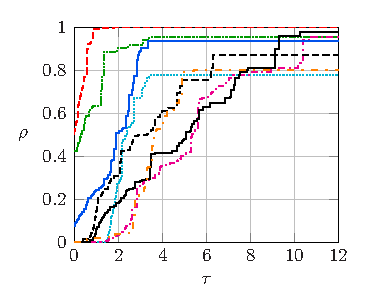
\includegraphics{lexample_fig1}
%  \caption{Example figure using external image files.}
%  \label{fig:testfig}
%\end{figure}
%
%\Cref{tab:foo} shows additional
%supporting evidence. 
%
%\begin{table}[htbp]
%\footnotesize
%\caption{Example table.}\label{tab:foo}
%\begin{center}
%  \begin{tabular}{|c|c|c|} \hline
%   Species & \bf Mean & \bf Std.~Dev. \\ \hline
%    1 & 3.4 & 1.2 \\
%    2 & 5.4 & 0.6 \\ 
%    3 & 7.4 & 2.4 \\ 
%    4 & 9.4 & 1.8 \\ \hline
%  \end{tabular}
%\end{center}
%\end{table}
%
%\lipsum[51]
%
%\section{Discussion of \texorpdfstring{{\boldmath$Z=X \cup Y$}}{Z = X union Y}}
%
%\lipsum[76]
%
%\section{Conclusions}
%\label{sec:conclusions}
%
%Some conclusions here.
%
%
%\appendix
%\section{An example appendix} 
%\lipsum[71]
%
%\begin{lemma}
%Test Lemma.
%\end{lemma}


\section*{Acknowledgments}
We would like to acknowledge the assistance of volunteers in putting
together this example manuscript and supplement.

\bibliographystyle{siamplain}
\bibliography{references}
\end{document}
